\documentclass{article}
\usepackage{CrimsonPro, eulervm}
\usepackage{amsmath, amssymb}
\usepackage{hyperref}

\begin{document}
\section{Generative Models}
\subsection{Dataset Selection and Preprocessing}

The dataset that will be used in this report is from \href{https://www.kaggle.com/datasets/gpiosenka/butterfly-images40-species}{Kaggle}. The dataset consists of 13594 total images, out of which 12594 are used for training, 500 for validation, and 500 for testing. Every set is partioned into 100 subdirectories, one for each species of butterfly or moth. [are the classes balanced, approximately?] The images are all in ${224 \times 224 \times 3}$ jpg format, which will be resized to ${64 \times 64 \times 3}$ for the purpose of this report. [is there a lot of noise or variation in the dataset?]

\begin{figure}[htb]
\centering	
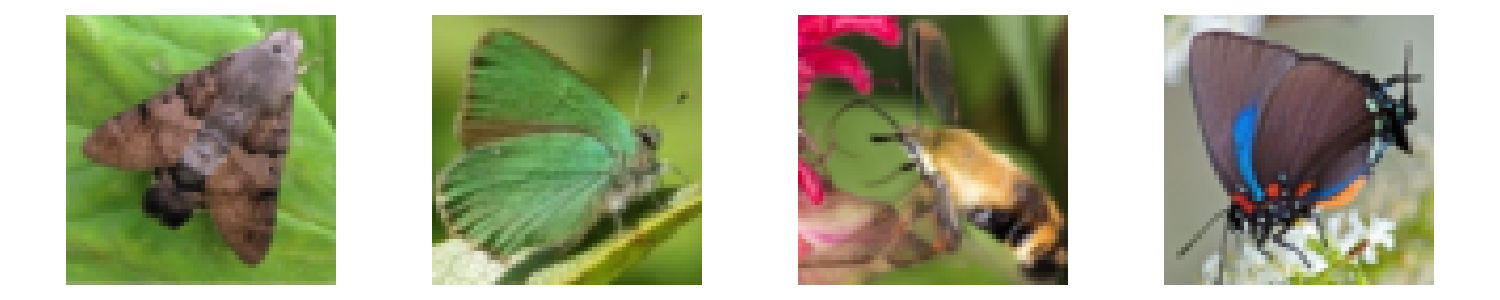
\includegraphics{pics/train_examples.png}
\caption{Sample Images from the Training Set}
\label{fig:train_examples}
\end{figure}

To give an idea of what images we are dealing with, we can look at 4 randomly selected examples from the training set, as shown in Figure \ref{fig:train_examples}.

\subsection{Convolutional Autoencoder}
\subsection{Variational Autoencoder}
\subsection{Generative Adversarial Network}
\subsection{Comparison}

\section{Sequence Modelling}
\subsection{Generalisation vs. Memorisation}
\subsection{Image-to-Text}
\subsection{Text-to-Image}
\subsection{Multi-Layer Architectures}
\end{document}
